\section{Stalag Might}\label{stalag-might}

Tags: PC Alias: Il bambino delle rocce Creatore: Francesco Curcio
Giocatore: Francesco Curcio Luogo: Bellavalle Razza: Nano Classe: Druido

\section{Stalag Might}\label{stalag-might-1}

\begin{center}\rule{0.5\linewidth}{0.5pt}\end{center}

\begin{figure}
\centering
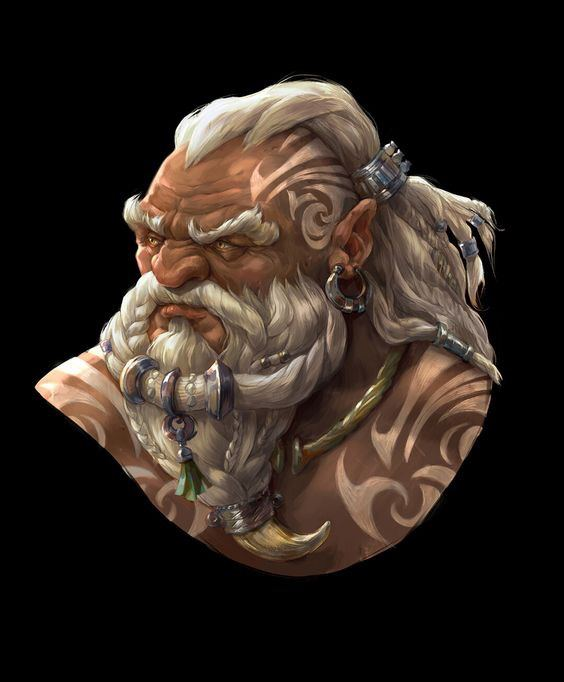
\includegraphics{2023-09-17_22.34.48.jpg}
\caption{2023-09-17 22.34.48.jpg}
\end{figure}

Informazioni Generali

Età:

Data di nascita:

Luogo di nascita: Lunacrest

Razza: Nano

Classe: Druido

Alleati:

Nemesi:

Alias:

Professione: Il bambino delle rocce

\begin{center}\rule{0.5\linewidth}{0.5pt}\end{center}

\subsection{1. Descrizione Generale}\label{descrizione-generale}

\begin{center}\rule{0.5\linewidth}{0.5pt}\end{center}

Stalag Might è un nano druido le cui origini sono radicate nelle
profondità di una montagna antica conosciuta come ``Lunacrest''. La sua
storia è intrecciata con il mistero di questa montagna, dove le energie
dell'antica luna scorrono nelle vene stesse della terra. Conosciuto tra
i druidi come il ``Bambino delle Rocce'', Stalag ha sempre mostrato una
connessione innata con le pietre e una passione per la geologia.

\begin{quote}
``Bella questa roccia''
\end{quote}

\subsection{2. Biografia}\label{biografia}

\begin{center}\rule{0.5\linewidth}{0.5pt}\end{center}

\subsubsection{2.1 Infanzia}\label{infanzia}

\begin{center}\rule{0.5\linewidth}{0.5pt}\end{center}

Stalag Might nacque nelle viscere di Lunacrest, portando con sé una
strana formazione rocciosa sulla mano sinistra, simile alle maestose
montagne circostanti. Questo segno innato attirò l'attenzione dei suoi
genitori, che lo condussero alla congrega dei druidi del Circolo della
Luna quando era ancora un neonato. Il giovane nano cresceva, diventando
noto tra i druidi come il ``Bambino delle Rocce''. La sua forza fisica e
la sua passione per la geologia lo resero un apprendista straordinario.

\subsubsection{2.2 Adolescenza}\label{adolescenza}

\begin{center}\rule{0.5\linewidth}{0.5pt}\end{center}

Durante gli anni della sua formazione, Stalag sviluppò un profondo
interesse per la metamorfosi, una delle abilità centrali dei druidi del
Circolo della Luna. A differenza dei suoi compagni, prediligeva
trasformarsi in piccoli animali, come topi, talpe e lucertole, per
esplorare fessure e cavità inaccessibili. Questa abilità gli consentiva
di scoprire gemme nascoste e segreti geologici, e raccontava avventure
vissute attraverso gli occhi di un piccolo animale.

\subsubsection{2.3 Età Adulta}\label{etuxe0-adulta}

\begin{center}\rule{0.5\linewidth}{0.5pt}\end{center}

Durnan Crystalbeard, il suo anziano maestro druido, riconoscendo il
talento e la dedizione di Stalag, gli regalò un geode speciale quando il
giovane nano compì sedici anni. Questo geode, inciso con simboli
druidici, divenne sia un focus per la sua magia che un santuario per
campioni di rocce e minerali rari. Dopo aver completato la sua
formazione con la congrega, Stalag sentì il richiamo dell'esplorazione e
del desiderio di scoprire montagne e formazioni rocciose leggendarie,
alla ricerca in particolare della pietra leggendaria nota come ``Il
Cuore della Luna''.

\subsection{3. Personalità}\label{personalituxe0}

\begin{center}\rule{0.5\linewidth}{0.5pt}\end{center}

Stalag Might è noto per la sua mente curiosa e la passione incrollabile
per la geologia. È un individuo tranquillo ma osservatore, sempre
desideroso di ascoltare le storie delle pietre e dei minerali che
incontra lungo il suo cammino. La sua connessione con la natura e il
mondo sotterraneo lo rende rispettoso nei confronti dell'ambiente
circostante.

Inoltre, la sua abilità unica di trasformarsi in creature più piccole
gli conferisce una prospettiva unica sulla vita e sull'esplorazione.
Stalag è affezionato ai suoi compagni druidi e considera ogni avventura
come un'opportunità per arricchire la sua comprensione delle meraviglie
naturali del mondo.

Stalag Might è guidato da una doppia missione: la sete di conoscenza
geologica e la ricerca dell'enigmatica ``Pietra della Luna''. Questo
equilibrio tra scienza e magia guida le sue azioni mentre viaggia
attraverso il mondo, pronta a esplorare e a svelare i segreti che
attendono sotto le rocce e nelle profondità della terra.

\subsection{4. Coinvolgimenti in Eventi
Recenti}\label{coinvolgimenti-in-eventi-recenti}

\begin{center}\rule{0.5\linewidth}{0.5pt}\end{center}

\href{Untitled\%20Database\%20da6a05127a584f75a0bd57df6960b00a.csv}{Untitled
Database}

\subsection{A. Scheda Personaggio}\label{a.-scheda-personaggio}

\begin{center}\rule{0.5\linewidth}{0.5pt}\end{center}

\href{Info\%20PG\%20c1cdb90ff3db4272965138ed0c53ac6e.csv}{Info PG}

\subsubsection{Statistiche e abilità}\label{statistiche-e-abilituxe0}

\begin{center}\rule{0.5\linewidth}{0.5pt}\end{center}

\href{Abilita\%CC\%80\%201e7ce6964e984b8d87837edf5c158b9c.csv}{Abilità}

\subsubsection{Lista magie}\label{lista-magie}

\subsection{B. Galleria Immagini}\label{b.-galleria-immagini}

\subsection{C. Descrizione Originale}\label{c.-descrizione-originale}

\begin{center}\rule{0.5\linewidth}{0.5pt}\end{center}

Stalag Mite nacque nelle profondità di una montagna antica, il cui cuore
pulsante era un rifugio segreto, scolpito nel tempo dai druidi del
Circolo della Luna. La montagna era chiamata ``Lunacrest'', e si diceva
che le sue vene fossero piene delle energie dell'antica luna. Fin dalla
sua nascita, Stalag mostrò una connessione innata con le rocce che lo
circondavano. La sua famiglia lo portò alla congrega dei druidi, tutti
nani come lui, quando era solo un neonato. Il motivo? Una particolare
increspatura sulla sua mano sinistra, una formazione rocciosa in
miniatura che assomigliava stranamente alle montagne che circondavano
Lunacrest. Man mano che Stalag cresceva, divenne noto tra i druidi come
il ``Bambino delle Rocce''. La sua forza, acquisita sollevando rocce e
aiutando nelle costruzioni all'interno della montagna, lo rese uno degli
studenti più fisicamente imponenti della sua età. Tuttavia, la sua
passione risiedeva nella geologia. Le rocce, i minerali, i cristalli:
tutto aveva una storia da raccontare, e Stalag voleva ascoltarle tutte.
Durante i suoi studi, Stalag scopriì un amore particolare per la
metamorfosi, una delle abilità cardine dei druidi del Circolo della
Luna. A differenza di molti dei suoi compagni druidi che preferivano
trasformarsi in creature grandi e potenti, Stalag aveva una predilezione
per piccoli animali: topi, talpe, lucertole e altri creature in grado di
infiltrarsi in crepe e cavità. Questa abilità gli permise di esplorare
profondità inaccessibili, scoprendo gemme nascoste e segreti geologici.
Era noto per raccontare storie di avventure vissute da un piccolo topo o
di passaggi segreti trovati sotto forma di lucertola. Il suo maestro, un
anziano druido chiamato Durnan Crystalbeard, gli regalò un geode
speciale quando Stalag compì sedici anni. Questo geode, decorato con
incisioni druidiche, non solo fungeva da focus per la sua magia, ma
conteneva anche un piccolo spazio all'interno, in cui Stalag conservava
campioni di rocce e minerali rari. Dopo aver completato la sua
formazione con la congrega, Stalag decise di esplorare il mondo. Voleva
vedere e studiare formazioni rocciose e montagne che la sua congrega
aveva solo menzionato nelle leggende. Ma oltre alla sua sete di
conoscenza, Stalag aveva anche un secondo obiettivo: trovare una pietra
leggendaria chiamata ``Il Cuore della Luna''. Si diceva che questa
pietra contenesse il potere della luna stessa e avrebbe potuto aumentare
enormemente i poteri di un druido del Circolo della Luna.

\begin{center}\rule{0.5\linewidth}{0.5pt}\end{center}

Nelle profondità di Lunacrest, il Circolo dei Druidi del Diamante Lunare
ha eretto il suo santuario. Questo circolo è composto principalmente da
nani, che vedono la luna come il massimo esempio di bellezza e forza
rocciosa. La luna, per loro, è la roccia madre, la pietra guida che
illumina il cielo notturno e dona forza e protezione al mondo
sottostante. Il santuario stesso è un capolavoro di architettura e
geologia. Le pareti e i soffitti sono scolpiti in forme che raffigurano
le fasi della luna e le sue influenze sulle rocce e sui minerali della
terra. In alcune camere, cristalli luminosi sono incastonati nel
soffitto, riflettendo la luce in modo da creare l'illusione di un cielo
stellato. Al centro del santuario c'è un grande altare circolare fatto
di una roccia che assomiglia al marmo lunare. Qui, durante le notti di
luna piena, i druidi si radunano per celebrare riti sacri e cantare inni
in onore della luna. Il circolo insegna che ogni roccia e minerale ha un
legame spirituale con la luna. Credono che la luna influenzi la
formazione delle rocce, il loro aspetto e le loro proprietà magiche.
Inoltre, ritengono che ogni druido possa attingere a questo legame
ancestrale attraverso la meditazione e le pratiche druidiche. La
formazione di un druido nel Circolo del Diamante Lunare non riguarda
solo la magia e la natura, ma anche la geologia. Si impara a leggere le
rocce, a comprenderne la storia e a utilizzare le loro energie in
sinergia con la magia druidica. Ogni druido è anche un geologo esperto,
capace di identificare minerali, predire terremoti e comprendere le
meraviglie nascoste sotto la superficie della terra. Stalag Mite, come
tutti gli altri druidi del circolo, ha trascorso anni ad affinare le sue
abilità geologiche e a comprendere il profondo legame tra le rocce e la
luna. Questa connessione lo ha aiutato a sintonizzarsi con la natura in
modi che altri druidi possono solo sognare, rendendolo uno dei membri
più rispettati del suo circolo nonostante la sua giovane età.
